\renewcommand\appendixname{Anhang}
\renewcommand\appendixpagename{Anhang}
\renewcommand\appendixtocname{Anhang}

\lohead{}

% Anhang Seite ohne Kopf- & Fußzeile
\appendix
\begingroup
\makeatletter
\let\ps@plain\ps@empty
\appendixpage
\makeatother
\endgroup

% Anhänge
\chapter{Anhang Elektronik}

\begin{figure}[htb]
    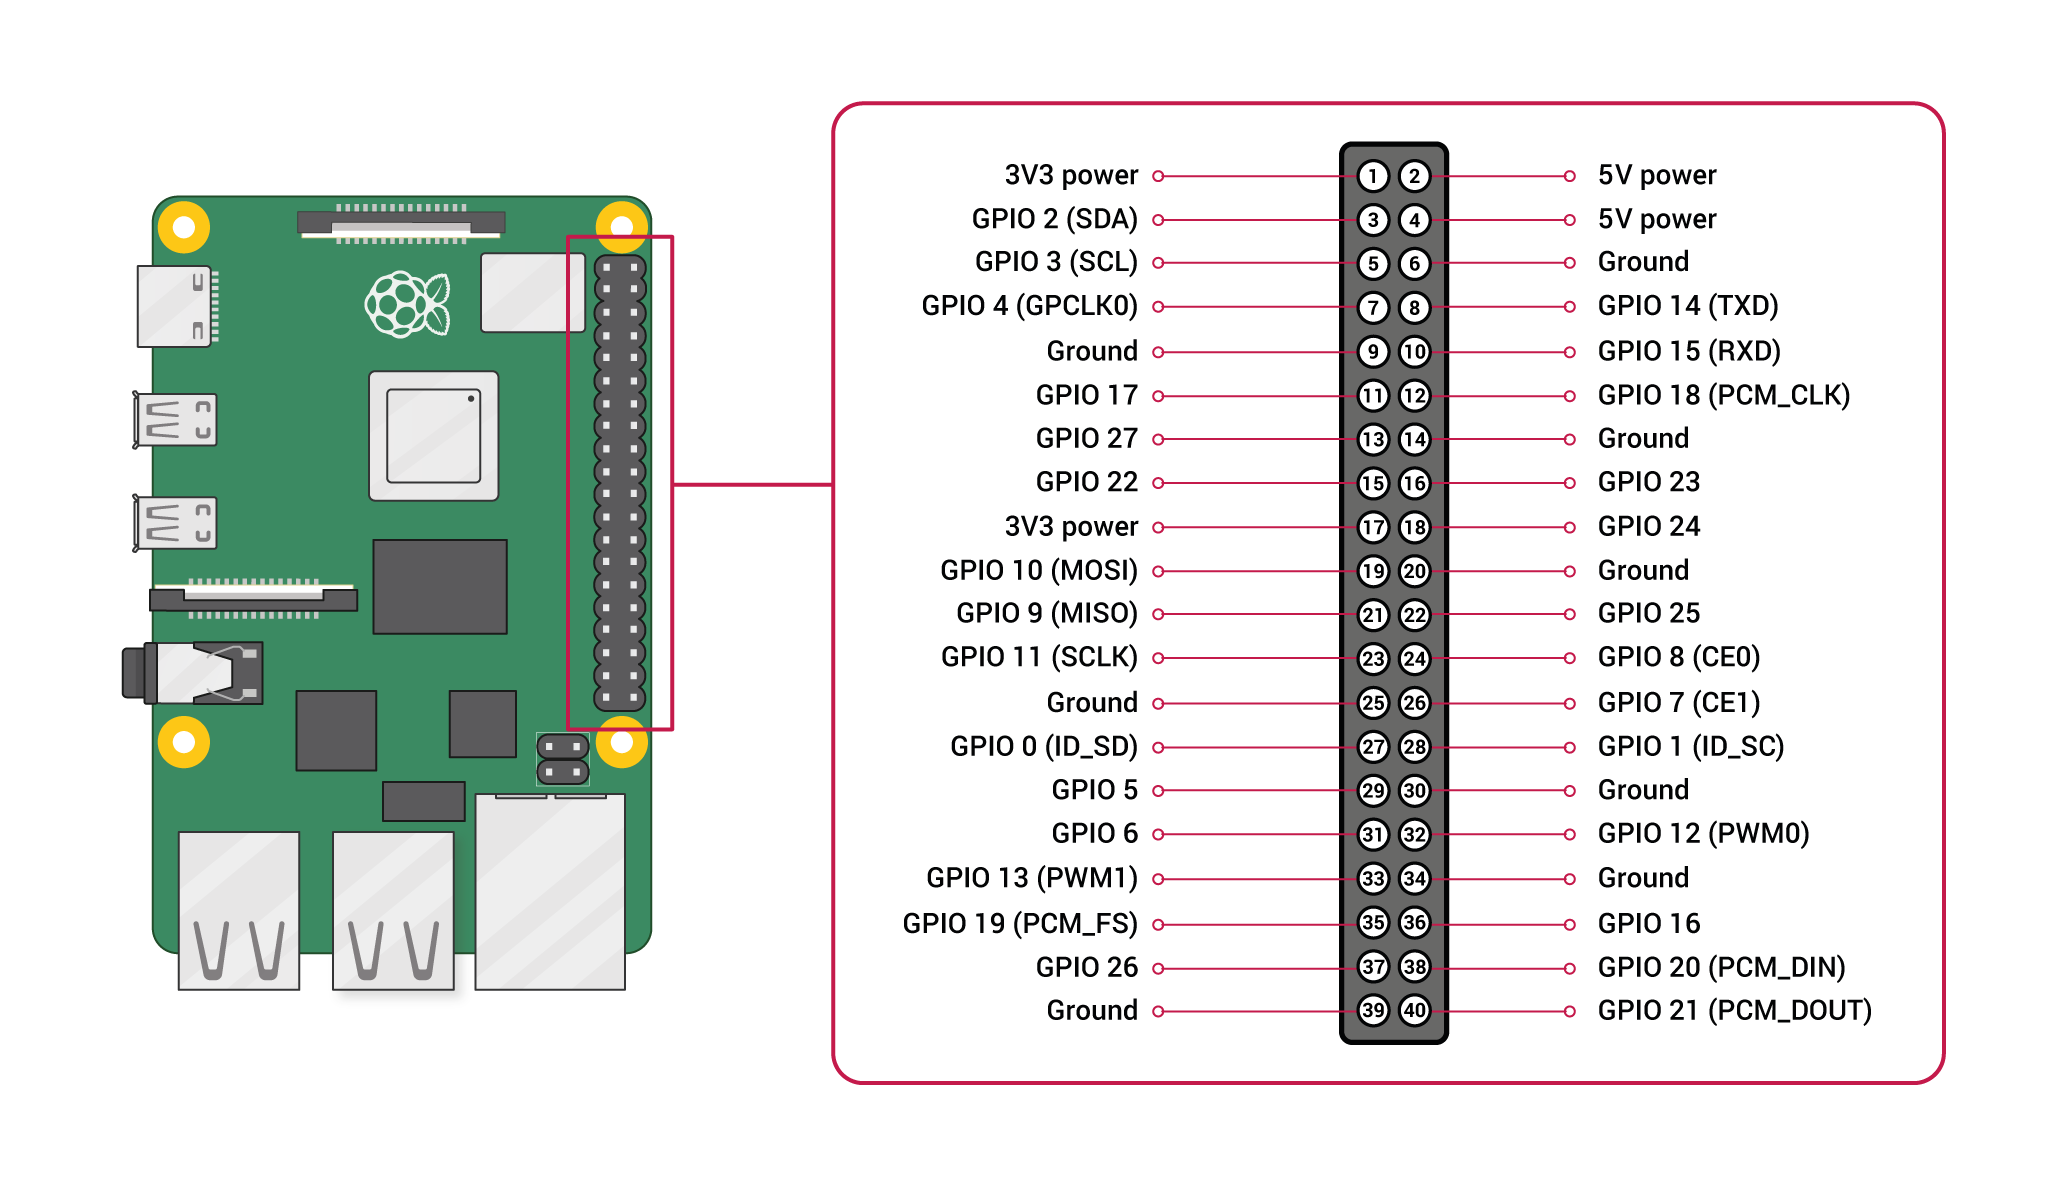
\includegraphics[scale=0.25]{fig/elektro/GPIO-Pinout-Diagram.png}
    {\par\raggedleft\footnotesize \tiny Quelle: \fullcite[][]{Raspberry-Pi-Pinout}}
    \caption{Pinout des Raspberry Pi}
\end{figure}

\begin{figure}[hb]
    \centering
    \includegraphics[scale=0.85,page=3]{fig/elektro/ATmega324PA.pdf}
    \caption{Pinout des ATmega324PA}
\end{figure}

\begin{figure}[hb]
    \centering
    \includegraphics[scale=0.85,page=318]{fig/elektro/ATmega324PA.pdf}
    \caption{Electrical characteristics des ATmega324PA}
\end{figure}

\begin{figure}[hb]
    \centering
    \includegraphics[scale=0.85,page=324]{fig/elektro/ATmega324PA.pdf}
    \caption{Speed grades des ATmega324PA}
\end{figure}

\begin{figure}[hb]
    \centering
    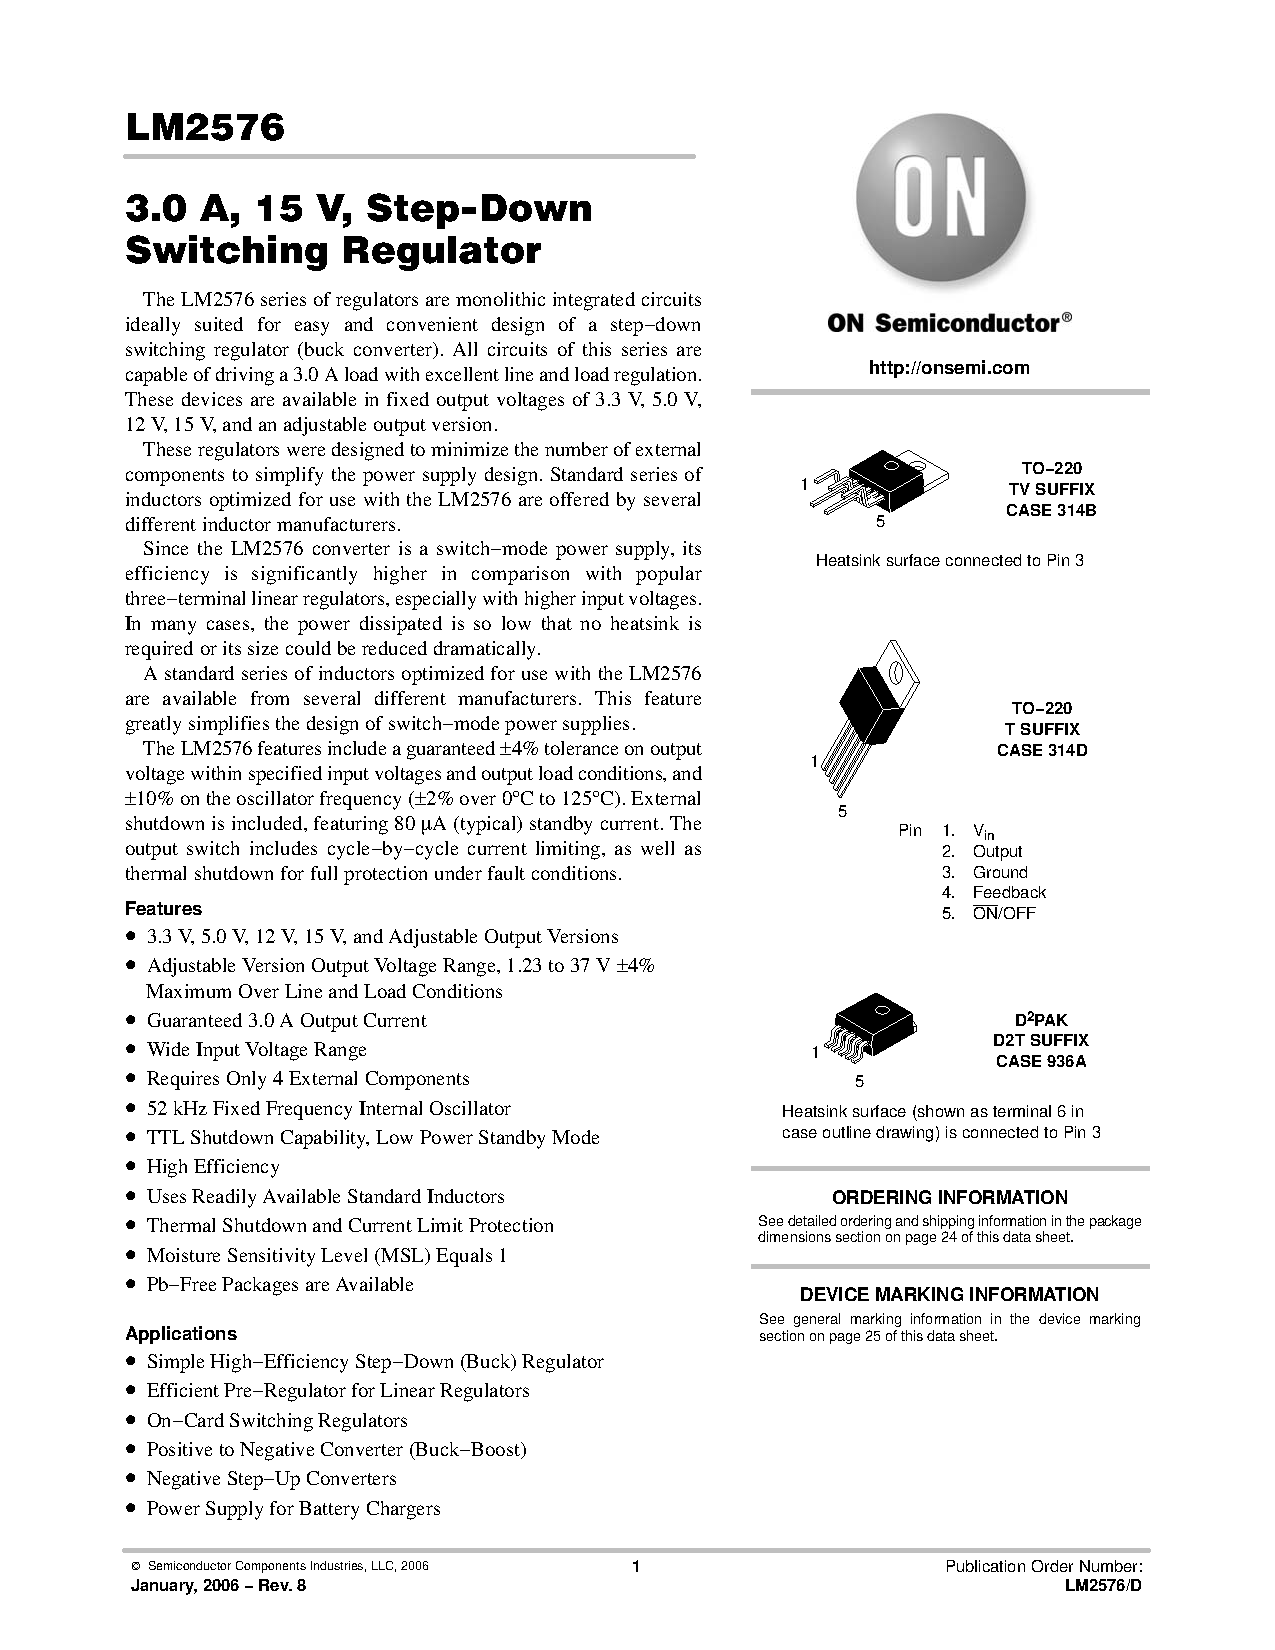
\includegraphics[scale=0.85,page=1]{fig/elektro/LM2576.pdf}
    \caption{Knappe Beschreibung des LM2576}
\end{figure}

\begin{figure}[hb]
    \centering
    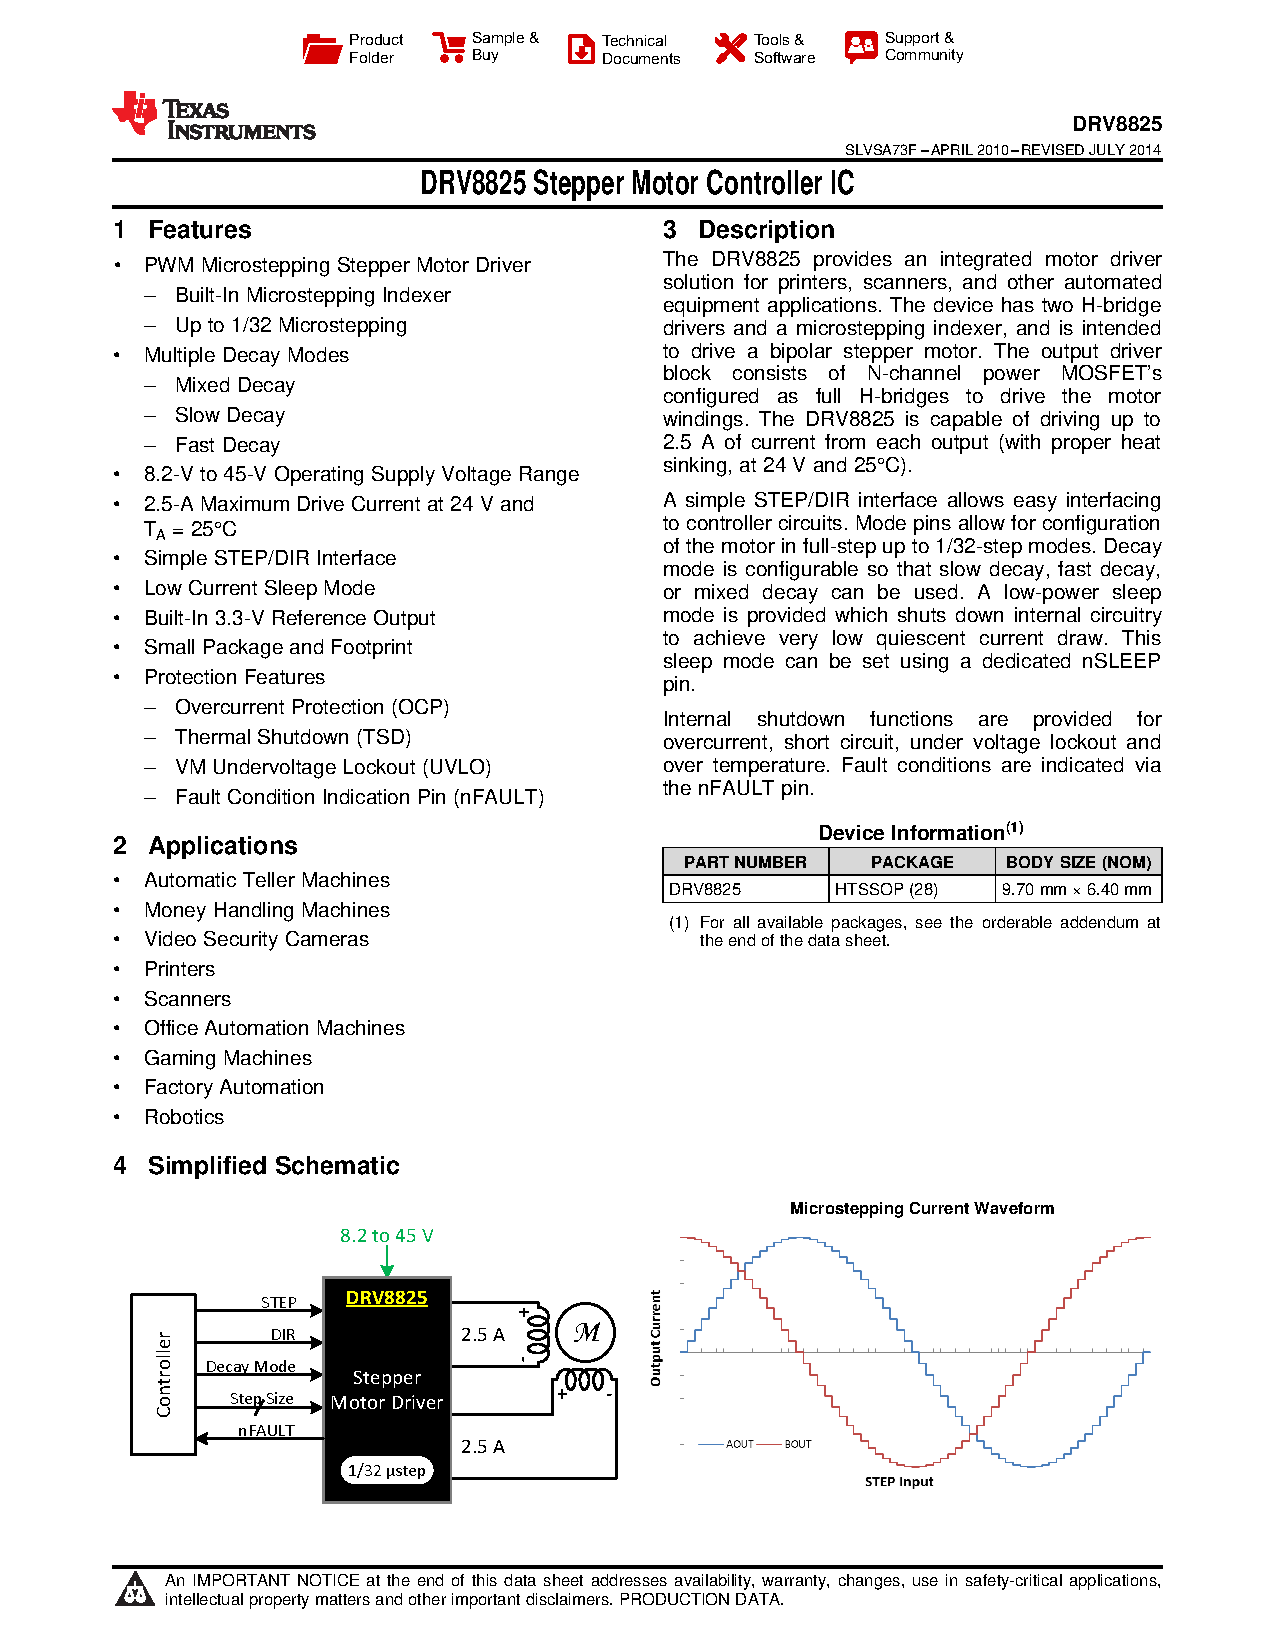
\includegraphics[scale=0.85,page=1]{fig/elektro/DRV8825.pdf}
    \caption{Knappe Beschreibung des DRV8825-Treibers}
\end{figure}

\begin{figure}[hb]
    \centering
    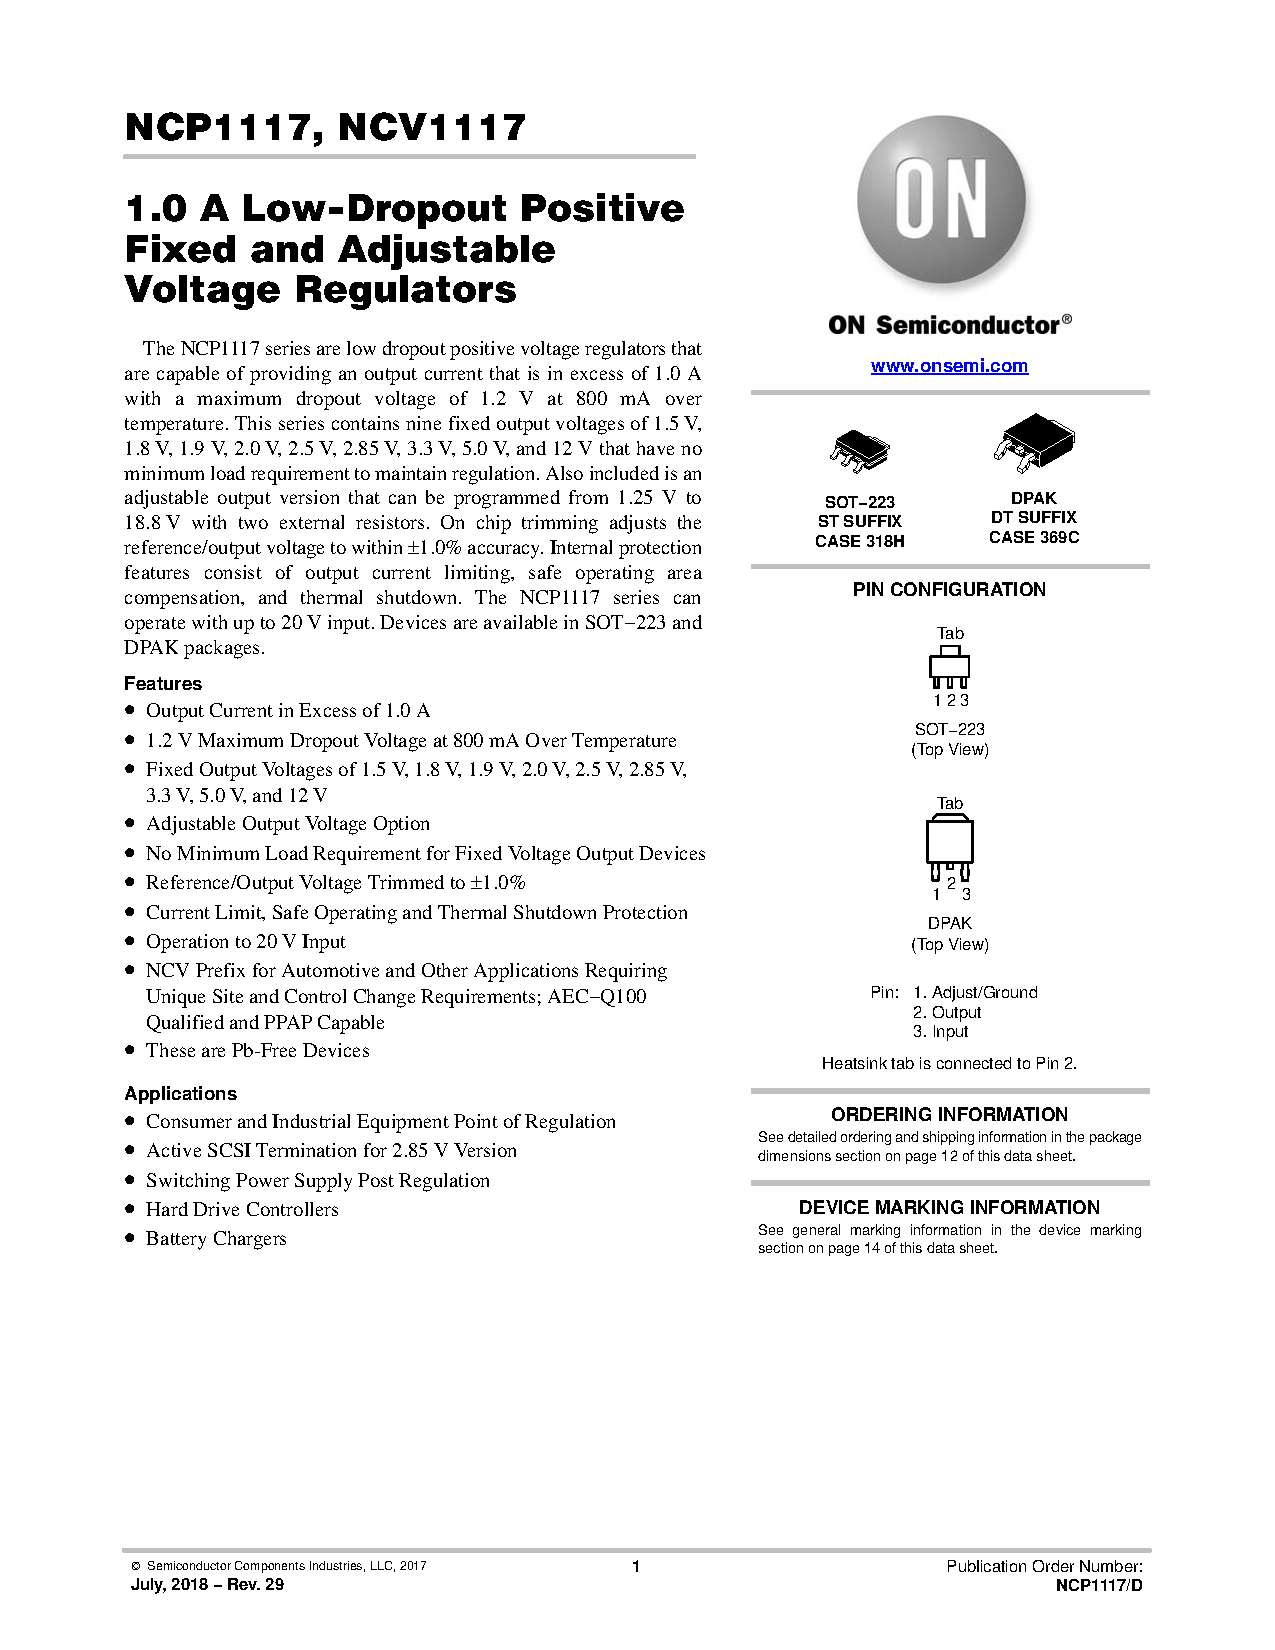
\includegraphics[scale=0.85,page=1]{fig/elektro/NCP1117-D.PDF}
    \caption{Knappe Beschreibung des NCP1117}
\end{figure}

\markboth{}{}    %end chapter

\printbibliography
\nocite{*}


\chapter{Abkürzungsverzeichnis}

\begin{acronym}
    \begin{singlespace}
        \acro{uC}[µC]{Mikrocontroller}
        \acro{UART}{Universal Asynchronous Receiver Transmitter}
        \acro{SPI}{Serial Peripheral Interface}
        \acro{SRAM}{Static random-access memory}
        \acro{EEPROM}{Electrically Erasable Programmable Read-Only Memory}
        \acro{I/O}{Ein-/Ausgabe}
        \acro{DIY}{Do it yourself}
        \acro{PWM}{Pulsweitenmodulation}
        \acro{DIP}{Dual in-line package}
        \acro{GND}{Ground, Masse}
        \acro{AC}{Wechselspannung}
        \acro{DC}{Gleichspannung}
        \acro{SN}{Schaltnetzteil}
        \acro{GPIO}{General Purpose Input Output}
        \acro{MOSFET}{Metall-Oxid-Halbleiter-Feldeffekttransistor}
        \acro{RPI}{Raspberry Pi}
        \acro{ESR}{Equivalent Series Resistance}
        \acro{USB}{Universal Serial Bus}
        \acro{RXD}{Received Data}
        \acro{LCD}{liquid crystal display}
        \acro{LED}{light-emitting diode}
        \acro{SMD}{Surface-mounted device}
        \acro{THT}{Through Hole Technology}
        \acro{TCP/IP}{Transmission Control Protocol/Internet Protocol}
		\acro{PC}{Personal computer}
		\acro{IDE}{Integrated development environment}
		\acro{GUI}{Graphical user interface}
		\acro{XML}{Extensible Markup Language}
		\acro{JSON}{JavaScript Object Notation}
		\acro{MVC}{Model-View-Controller}
		\acro{CSS}{Cascading Style Sheets}
		\acro{CSV}{Comma-separated values}
		\acro{ASCII}{American Standard Code for Information Interchange}
		\acro{CRC}{Cyclic redundancy check}
		\acro{UML}{Unified Modeling Language}
		\acro{jSSC}{Java Simple Serial Connector}
		\acro{Config}{Configuration}
		\acro{Stats}{Statistics}
		\acro{AutoDeal}{Automatic Deal}
		\acro{JVM}{Java virtual machine}
        \acro{PLA}{Polylactide}
        \acro{ABS}{Acrylnitril-Butadien-Styrol-Copolymer}
        \acro{GRP}{Glass Reinforced Plastic}
        \acro{ASA}{Acrylnitril-Styrolacrylat}
        \acro{PET}{Polyethylenterephthalat}
        \acro{GRP}{Glass Reinforced Plastic}
        \acro{TO}{Transistor Single Outline}
        \acro{SOD}{Small Outline Diode}
        \acro{SOT}{Small Outline Transistor}
    \end{singlespace}
\end{acronym}

\printacronyms
\listoffigures
\listoftables
\lstlistoflistings